\documentclass[11pt,spanish]{article}

\usepackage[a6paper, landscape,
	left=1cm, top=1cm, right=1cm, bottom=1.5cm
]{geometry}
%\usepackage[a4paper, margin=3cm]{geometry}
\usepackage{babel}
\usepackage{xltxtra}
\usepackage{grid-system}
\usepackage{multicol} % simpler than grid for lots of cases
\usepackage{hyperref}
\usepackage{xcolor}
\usepackage{graphicx}
\usepackage[export]{adjustbox}
\usepackage{fancyhdr}
\usepackage{listings}

\setmainfont{Comic Sans MS}
%\setmathfont{eulervm}
%\lstset{basicstyle=\footnotesize\ttfamily}
\lstset{basicstyle=\footnotesize\setmainfont{DejaVu Sans Mono}}

\definecolor{verletblue}{HTML}{487AD8}
\definecolor{verletgreen}{HTML}{37DE88}
\definecolor{verletcyan}{HTML}{1AFBFF}

\fancyhead{}
\fancyfoot{}
\fancyfoot[RO]{{\footnotesize \thepage\ de\ \pageref*{lastpage}}}
\renewcommand{\headrule}{}
%\renewcommand{\footrule}{\vbox to 0pt{\hbox to\headwidth{\dotfill}\vss}}
% XXX should find way to use only one right aligned rule...
\renewcommand{\footrule}{{\footnotesize \rule{\textwidth - 5ex}{0pt}\rule{5ex}{1pt}\vss}}
\pagestyle{fancy}

\newcommand{\fr}[1]{%
	\begin{flushright}
		#1
	\end{flushright}
}
%row space
\newcommand{\rowsp}[1][1em]{\vspace{#1}}
\newcommand{\hone}[1]{{\rowsp[0.3em]\noindent\Large #1 \rowsp[0.3em]}}
\newcommand{\htwo}[1]{{\rowsp\noindent\large #1 \rowsp}}
\newcommand{\htworuler}[1]{{%
	\rowsp\noindent\Large #1%
	\\ {\color{verletgreen}\noindent\rule{\textwidth + 2em}{0.5em}}\rowsp%
}}
\newcommand{\hthree}[1]{{\rowsp\noindent\large #1 \rowsp[0.5em]}}
\newcommand{\hfour}[1]{{\rowsp\large #1 \rowsp[0.5em]}}
\newcommand{\for}[1]{{#1 \rowsp}}
\newcommand{\signline}{\rule{\textwidth}{1pt}}
\newcommand{\emptycell}[1][1]{\begin{Cell}{#1}\ \end{Cell}}
%page with single text horizontally and vertically centered
\newcommand{\displaypage}[1]{%
\
\vspace{\stretch{1}}
\begin{center}
\hone{#1}
\end{center}
\vspace{\stretch{1}}
}

%=======================
% specific to presentations
%\newcommand{\myitm}{aoeuaeou}
\newcommand{\myitm}[1]{\begin{itemize}#1\end{itemize}}

\newcommand{\mydesc}[1]{%
	\begin{description}
	\setlength\itemsep{0em}%
	#1
	\end{description}
}
\newcommand{\pros}{\item[pros:]}
\newcommand{\cons}{\item[cons:]}

\setlength{\parindent}{0pt}
\setlength{\parskip}{1ex plus 0.5ex minus 0.2ex}

%=======================

%\renewcommand{\emph}[1]{\emph{#1}}

\title{Diseño e implementación: Prometheus node exporter en C para OpenBSD}
\author{Abel Camarillo $<$acamari@verlet.org$>$}

\begin{document}

\maketitle
\thispagestyle{empty}

\newpage

\hone{Agenda}

\myitm{
	\item ¿Quién soy?
	\item ¿Qué es?
	\item ¿Por qué?
	\item ¿Cómo?
}

\newpage %===============
\hone{¿Quién soy?}
\begin{Row}
\begin{Cell}{2}
\myitm{
	\item Desarrollador de software desde el 2008 - OpenBSD, perl, C, sh, js
	\item Lead developer en Neuroservices Communications durante 6 años.
	\item Desarrollador freelance desde el 2015 - Verlet.
	\item Maintainer de 21 paquetes en el árbol oficial de OpenBSD -
	\href{http://openports.se/bbmaint.php?maint=acamari@verlet.org}{
	      http://openports.se/bbmaint.php?\textbackslash{} maint=acamari@verlet.org}
	\item Interés en UNIX, poesía, $\sim$arte$\sim$, cocina, etc...
}
\end{Cell}

\begin{Cell}{1}
\ \\ %XXX so image hasn't its bottom to baseline
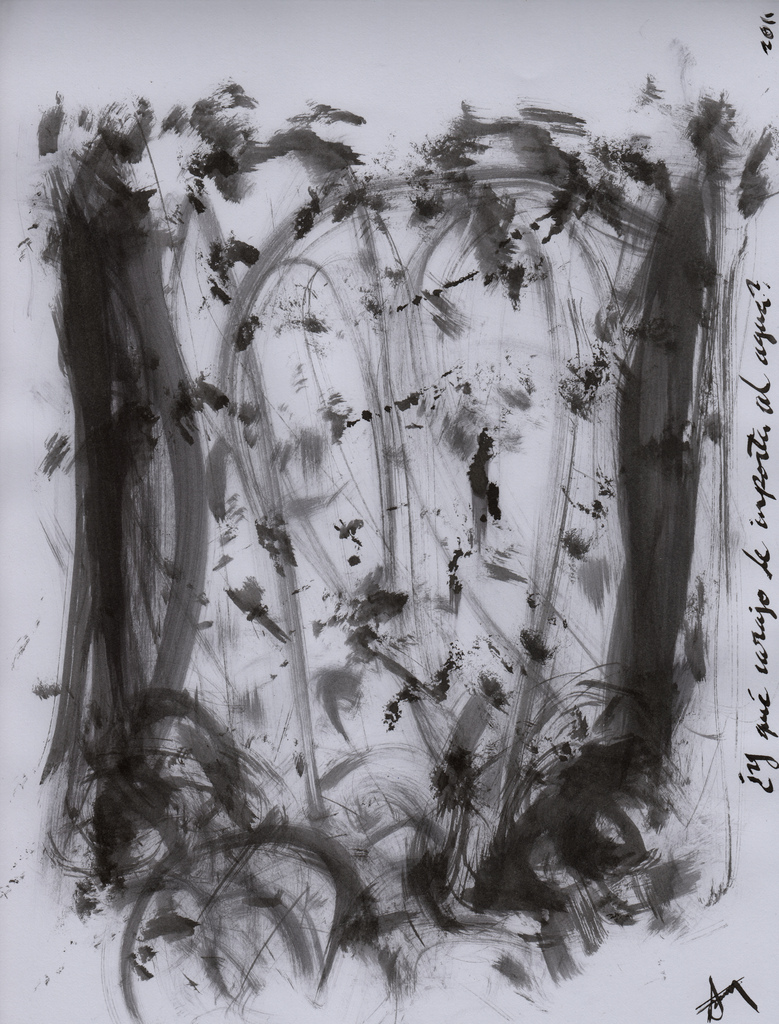
\includegraphics[width=\textwidth]{img/carajo}
\fr{ {\tiny ¿Y qué carajo\\
le importa al agua? - 2011} }
\end{Cell}

\end{Row}


\newpage %===============
\hone{¿Qué es?}

\myitm{
	\item ¿Qué es Prometheus?
	\item ¿Qué es OpenBSD?
	\item ¿Qué es C?
	\item ¿Qué es un exporter?
	\item ¿Qué es el node\_exporter?
}

\newpage %===============
\displaypage{Arquitectura original}

\newpage %===============
\begin{center}
	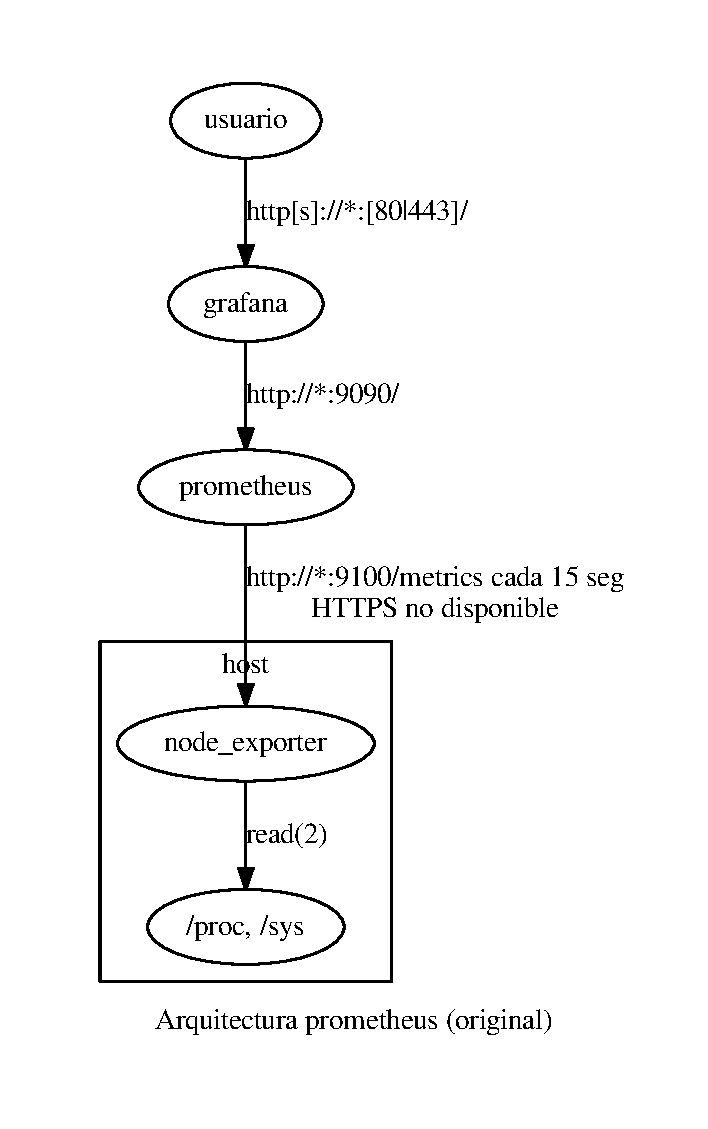
\includegraphics[keepaspectratio=true,width=\textwidth,height=\textheight]{img/pronodebsd/arq}
\end{center}

\newpage %===============
\hone{¿Por qué?}

Quiero monitorear mi router.
\myitm{
	\item Ubiquiti EdgeRouter-Lite (dual octeon@500mhz)
	\item OpenBSD-6.5/mips64 (dual-endianess, OpenBSD escogió BE)
	\item go sólo disponible en i386 y amd64
	\item ¿Por qué no portar go?: go-bootstrap
	\item Aunque hubiera go:
		\myitm{
			\item node\_exporter incompleto en *BSD (/proc, /sys)
		}
	\item Alternativas:
		\myitm{
		\item prometheus\_sysctl\_exporter (FreeBSD)
		\item Incompatible con node\_exporter
		}
}

\newpage %===============
\hone{¿Por qué?}

Sí, pero, ¿en C?
\myitm{
\item No hay /proc, /sys.
\item Disponibilidad de sysctl(3)
\item Acceso a unveil(2), pledge(2)
\item Sí hay perl en OpenBSD base, pero no BSD::Sysctl.
	Además third-party. Sino: perlxs, (un)pack, etc...
\item No hay python en OpenBSD base. Acceso sysctl indefinido.
\item ¿nodejs?: jajajaja
}

\newpage %===============
\hone{¿Cómo?}

\htwo{Diseño}

\myitm{
\item Formato de intercomunicación
\item Seguridad
\item Arquitectura
\item Integración
\item Simplicidad
\item Interfaz
}

\newpage %===============
\hone{Formato de intercomunicación}

V4. Definido en github de prometheus (\textbackslash{} agregados para legibilidad):

\href{https://github.com/prometheus/docs/blob/master/content/docs/instrumenting/exposition_formats.md}{\tiny https://github.com/prometheus/docs/blob/master/content/docs/instrumenting/exposition\_formats.md}

Ejemplo:
\begin{lstlisting}
$ curl http://*:9100/metrics;
...
# HELP node_forks_total Total number of forks.
# TYPE node_forks_total counter
node_forks_total 1.8757377e+07
# HELP node_load1 1m load average.
# TYPE node_load1 gauge
node_load1 1
# HELP node_load15 15m load average.
# TYPE node_load15 gauge
node_load15 1.37
# HELP node_load5 5m load average.
# TYPE node_load5 gauge
node_load5 1.15
# HELP node_uname_info Labeled system information as provided by   \
	the uname
system call.
# TYPE node_uname_info gauge
node_uname_info{domainname="(none)",machine="x86_64",nodename="db4"\
    ,release="4.15.12-x86_64-linode105",sysname="Linux",\
    version="#1 SMP Thu Mar 22 02:13:40 UTC 2018"} 1
# HELP process_cpu_seconds_total Total user and system CPU time \
    spent in seconds.
# TYPE process_cpu_seconds_total counter
process_cpu_seconds_total 2111.27
# HELP node_cpu_seconds_total Seconds the cpus spent in each mode.
# TYPE node_cpu_seconds_total counter
node_cpu_seconds_total{cpu="0",mode="idle"} 2.980243359e+07
node_cpu_seconds_total{cpu="0",mode="iowait"} 8497.06
node_cpu_seconds_total{cpu="0",mode="irq"} 0
node_cpu_seconds_total{cpu="0",mode="nice"} 20709.44
\end{lstlisting}

\newpage %===============
\hone{Formato de intercomunicación}

\myitm{
\item Una métrica puede tener varios valores si hay etiquetas
\item Las etiquetas pueden tener longitud arbitraria
\item Etiquetas pueden variar entre ejecuciones: fs nuevos, tarjetas
	de red o IPs entran y salen, etc
\item Se observaron crasheos en las condiciones anteriores
}
\newpage %===============

\hone{Seguridad}

node\_exporter:
\myitm{
\item Amplia superficie de ataque: sockets (DOS), http parsing
\item Mucha gente lo corre como root
\item Sin soporte HTTPS
}

\newpage %===============

\hone{Seguridad}

pronodebsd:
\myitm{
\item Sin web server: desplaza superficie de ataque a otra capa
\item No analiza entradas externas (aparte de argumentos de inicio y
	salida de sysctl(3))
\item ¿Si sysctl regresa basura? Hay problemas más graves
\item \lstinline|unveil(\"/var/www/pronodebsd/", "rw");|
	\lstinline|unveil(NULL, NULL);|
\item Usuario sin privilegios
}

\newpage %===============
\displaypage{Arquitectura pronodebsd}

\newpage %===============
\begin{center}
	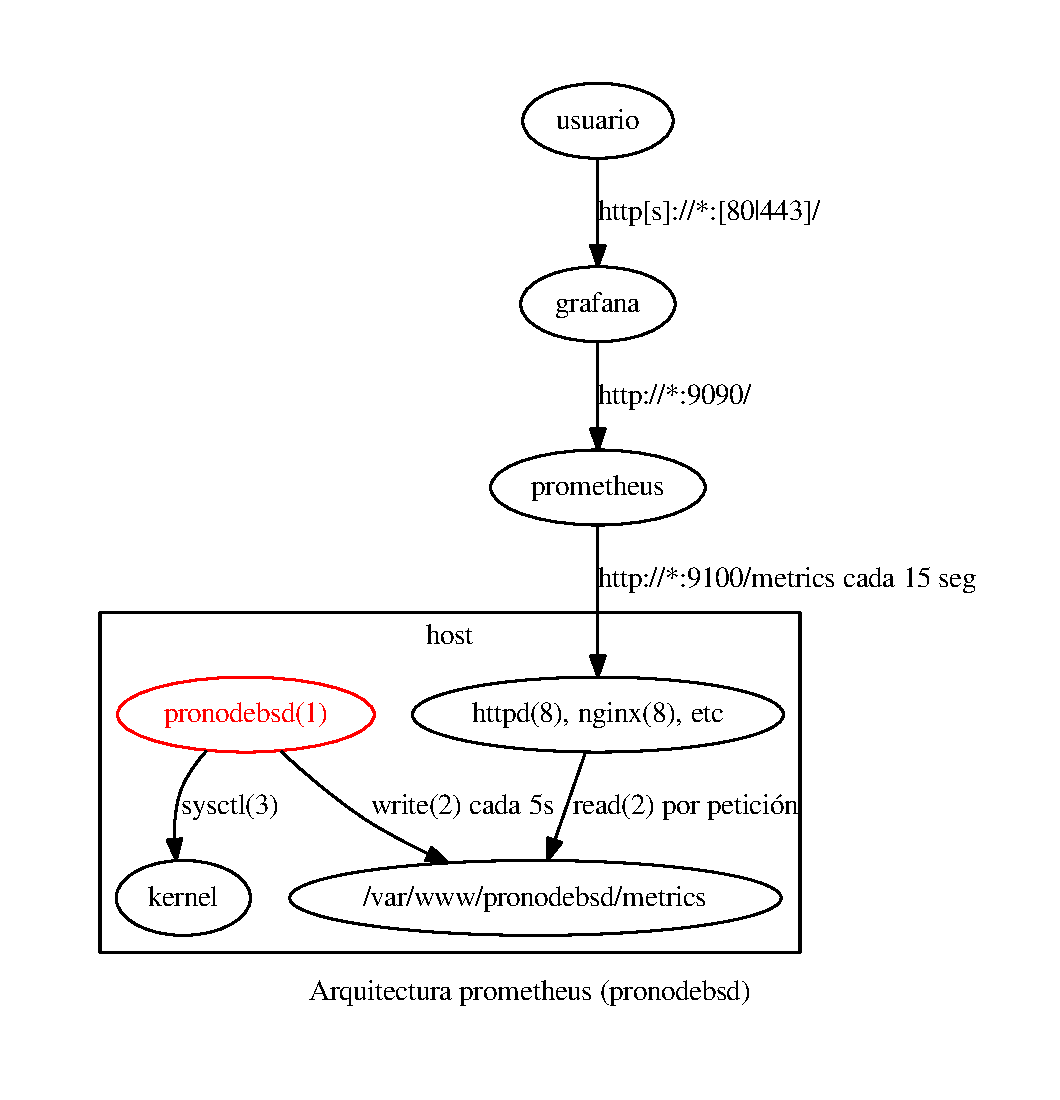
\includegraphics[keepaspectratio=true,width=\textwidth,height=\textheight]{img/pronodebsd/arq-2}
\end{center}

\newpage %===============
\hone{Integración}

\myitm{
\item Logueo tradicional: syslog, newsyslog, logrotate, etc
\item Manejo de señales: SIGHUP, SIGINT, etc
\item Manejo atómico de archivos:
	\myitm{
	\item No queremos escribir archivo metrics a medias, porque
		en el resto del stack no se podría distinguir la falta
		de métrica vs archivo a medias
	\item Usar archivo temporal /var/www/pronodebsd/.metrics
	\item \lstinline|rename("./.metrics", "./metrics")|
	}
}

\newpage %===============
\hone{Simplicidad}

\myitm{
\item No hay necesidad de recalcular stats < 5seg
\item Es el tiempo de refresco de muchos parámetros de kernel: loadavg,
	temperatura, etc
\item Facilidad para añadir collectors
\item Manejo de memoria de heap fuera de los collectors, prevenir leaks.
	No regresar memoria estática, ni global, ni malloc(3) (sin free(3)
	léxico) dentro de collectors
}

\newpage %===============
\hone{Interfaz}

\begin{lstlisting}
pronodebsd [-d dir] [-s secs] [-f]
	-d directory (/var/www/pronodebsd)
	-s seconds (5)
	-f foreground, ignore -s and -d and print once to stdout
\end{lstlisting}

\newpage %===============
\hone{¿Cómo?}

\htwo{Implementación}

\myitm{
\item Estructuras de datos
\item Collectors
\item Status
}

\newpage %===============
\hone{Implementación}

pronodebsd.c:
\begin{lstlisting}
struct mresult {
	int	labelsz;	/* size allocated for labels */
	int	nlabelsz;	/* size should be allocated for labels */
	char	*label;		/* one or more labels */
	double	value;
};
\end{lstlisting}
\newpage %===============
\hone{Implementación}

pronodebsd.c:
\begin{lstlisting}
enum METRIC_TYPES { MTYPE_UNTYPED = 0, MTYPE_COUNTER, MTYPE_GAUGE,
			MTYPE_HISTOGRAM, MTYPE_SUMMARY };

static struct metrics_t {
	char	*name;
	char	*help;
	enum METRIC_TYPES	type;
	/* use only one of collector or collectorv */
	int	(*collector)(double *, char **);
	int	(*collectorv)(struct mresult *, int, char **, int *);
	int	nelem; /* number of elements the collector returned */
	/* storage for collectors that return complex results */
	struct mresult	*mres;
};
\end{lstlisting}

\newpage %===============
\hone{Implementación}

pronodebsd.c:
\begin{lstlisting}
static struct metrics_t metrics[] = {
	...
	{ "node_intr_total", "Total number of interrupts serviced.",
	    MTYPE_GAUGE, intr_collector, NULL, 0, NULL },
	{ "node_uname_info", "Labeled system information as "
	     "provided by the uname system call.", MTYPE_GAUGE, NULL,
	     uname_collector, 0, NULL },
	{ NULL, NULL, 0, NULL, NULL, 0, NULL }
};
\end{lstlisting}

\newpage %===============
\hone{Implementación}

sysctl.c:
\begin{lstlisting}
#include <sys/types.h>
#include <sys/sysctl.h>
#include <sys/vmmeter.h>
#include <uvm/uvmexp.h>

#include <stdlib.h>
#include <string.h>
#include <errno.h>

#include "sysctl.h"

static int
uvmexp_collector(struct uvmexp *uvmexp, char **err)
{
	size_t	sz = sizeof *uvmexp;
	int	mib[] = { CTL_VM, VM_UVMEXP };

	if (sysctl(mib, sizeof mib / sizeof mib[0], uvmexp, &sz,
		   NULL, 0) == -1) {
		*err = strerror(errno);
		return -1;
	}
	return 0;
}

int
intr_collector(double *result, char **err)
{
	struct uvmexp	uvmexp;

	if (uvmexp_collector(&uvmexp, err) == -1) {
		return -1;
	}

	*result = uvmexp.intrs;
	return 0;
}
\end{lstlisting}

\newpage %===============
\hone{Implementación}

sysctl.c:
\begin{lstlisting}
#include <sys/utsname.h>
static int
uname_collector(struct mresult *mres, int nelem, char **err,
	int *newnelem)
{
	struct utsname	un;
	char buf[1024] = "";
	/* max number of elements this func will return */
	const int maxelem = 1;
	int c;

	*newnelem = maxelem;
	if (nelem < maxelem) {
		return 0;
	}

	if (uname(&un) == -1) {
		*err = strerror(errno);
		return -1;
	}

	c = snprintf(buf, sizeof buf,
			"domainname=\"(none)\","
			"machine=\"%s\","
			"nodename=\"%s\","
			"release=\"%s\","
			"version=\"%s\"",
			un.machine,
			un.nodename,
			un.release,
			un.version);
	if (c < 0) {
		*err = "snprintf";
		return -1;
	}

	mres->nlabelsz = c + 1; /* add \0 */
	if (mres->labelsz < mres->nlabelsz) { /* not enough space */
		return 0;
	}

	mres->labelsz = mres->nlabelsz;
	mres->value = 1;
	strlcpy(mres->label, buf, mres->labelsz);
	return 1;
}
\end{lstlisting}



\newpage %===============
\hone{Status}

Falta:
\myitm{
\item Escribir archivo real
\item Loop de actualización
\item Muchísimas métricas, es trabajo simple pero tedioso
\item Integración con «init» de OpenBSD rc(8)
\item Hacer port, para poder hacer pkg\_add pronodebsd
\item manpage, README de instalación
}

\newpage %===============
\displaypage{¿Preguntas?}

\label{lastpage}
\end{document}
